\documentclass[xcolor=table]{beamer}
\usetheme{boxes}

\usepackage[utf8]{inputenc}
\usepackage[T1]{fontenc}
\usepackage[brazil]{babel}
\usepackage{amsmath}
\usepackage{amsfonts}
\usepackage{amssymb}
\usepackage{graphicx}
\usepackage{booktabs}
\usepackage{adjustbox}
\usepackage{multirow}

\author{Bruno Ferrari Guide}
\title{Classificador Bayesiano Ingênuo para o Acento do PB}
%\subtitle{}
%\logo{}
\institute{Orientador: Marcelo Barra Ferreira\\ Departamento de Linguística - FFLCH - USP}
\date{17 de maio de 2016}
%\subject{}
%\setbeamercovered{transparent}
%\setbeamertemplate{navigation symbols}{}

\begin{document}
	%1
	\maketitle
%%%%%%%%%%%%%%%%%%%%%%%%%%%%%%%%%%%%%%%%%%
	\section{Introdução}
	%2
	\begin{frame}
		\frametitle{Introdução}
		\begin{itemize}
			\item Tópicos dessa apresentação:\\
			\begin{itemize}
				\item Objetivos\\
				\item Sobre o acento\\
				\item O Classificador Bayesiano Ingênuo\\
				\item Resultados\\
				\item Perspectivas\\
			\end{itemize}
		\end{itemize}
	\end{frame}

%%%%%%%%%%%%%%%%%%%%%%%%%%%%%%%%%%%%%%%%%%%%%

	\section{Objetivos}
	%3
	\begin{frame}
		\frametitle{Objetivos}
		\begin{itemize}
			\item A partir da criação de modelos probabilísticos, eu pretendo apresentar uma discussão sobre o comportamento do acento no PB.\\
			\item Os modelos são baseados em corpus e podem trazer à tona algumas características quantitativas sobre esse comportamento.\\
			\item Os modelos retornam as probabilidades de uma determinada palavra pertencer a alguma categoria acentual (Oxítona, Paroxítona, Proparoxítona) e a partir disso é possível discutir os erros e os acertos de um modelo.\\
		\end{itemize}
	\end{frame}


%%%%%%%%%%%%%%%%%%%%%%%%%%%%%%%%%%%%%%%%%%%%%

	\section{Sobre o Acento}
	\begin{frame}
		\centering \textbf{Sobre o acento\\}
	\end{frame}
	%4
	\begin{frame}
		\frametitle{Sobre o Acento - 2 tendências}
		\begin{itemize}
			\item O acento no português brasileiro (quase) sempre ocupa uma das três últimas posições da palavra, criando as três categorias acentuais: Oxítona, Paroxítona, Proparoxítona.
			\item Duas tendências dão conta da maioria das palavras do PB:
			\begin{itemize}
				\item Caso a sílaba final seja pesada, a palavra é oxítona.\\
				\item Caso a sílaba final seja leve, a palavra é paroxítona.\\
			\end{itemize}
		\end{itemize}
	\end{frame}
	%5
	\begin{frame}
		\frametitle{2 tendências?}
		\begin{itemize}
			\item Problemas com palavras oxítonas terminadas em sílaba leve, como \textit{caqui, urubu}\\
			\item Problemas com paroxítonas terminadas em sílaba pesada, como em \textit{mártir, câncer, difícil}.\\
			\item Problemas com as proparoxítonas de modo geral.\\
			\item O acento é regular, porém tem irregularidades.\\
			\item O acento é irregular, porém tem regularidades.\\
		\end{itemize}

	\end{frame}	
%%%%%%%%%%%%%%%%%%%%%%%%%%%%%%%%%%%%%%%%%%%%%%%%%%%%%
	\section{O classificador Bayesiano Ingênuo}
	
	\begin{frame}
		\frametitle{Sobre modelos probabilísticos}
		\begin{itemize}
			\item Modelo é uma representação formal de um objeto.\\
			\item As vezes, o objeto possui comportamento imprevisível.\\
			\item Na matemática, a área que lida com a imprevisibilidade (ou seja, que a quantifica e formaliza) é a probabilidade.\\
			\item Existem muitas formas de tentar formalizar essa imprevisibilidade, cada uma possui suas vantagens e desvantagens.\\
		\end{itemize}
	\end{frame}
	%6	
	\begin{frame}
		\centering \textbf{O classificador Bayesiano Ingênuo\\}
	\end{frame}
	\begin{frame}
		\frametitle{Classificador}
		\begin{figure}
\centering
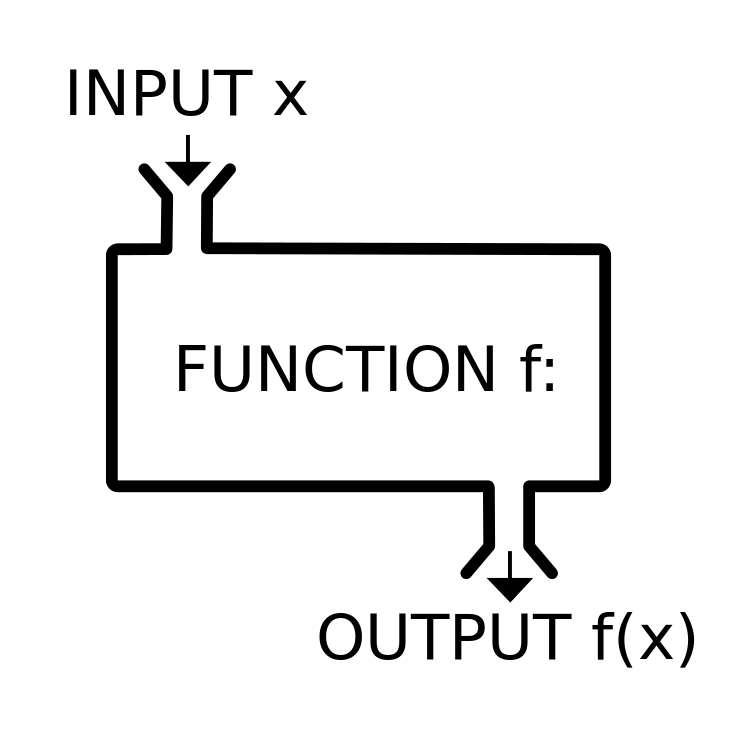
\includegraphics[width=0.5\linewidth,height=0.5\textheight]{funcao-esquema}
\caption{Um classificador é uma função}
\label{fig:funcao-esquema}
\end{figure}
	
	\end{frame}
	\begin{frame}
		\frametitle{Classificador}
		\begin{figure}
\centering
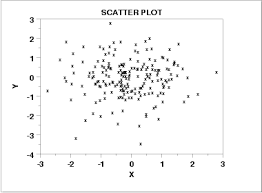
\includegraphics[width=0.7\linewidth]{classes-feio}
\caption{Em que temos observações como input}
\label{fig:classes-feio}
\end{figure}

	\end{frame}
	\begin{frame}
		\frametitle{Classificador}
		\begin{figure}
\centering
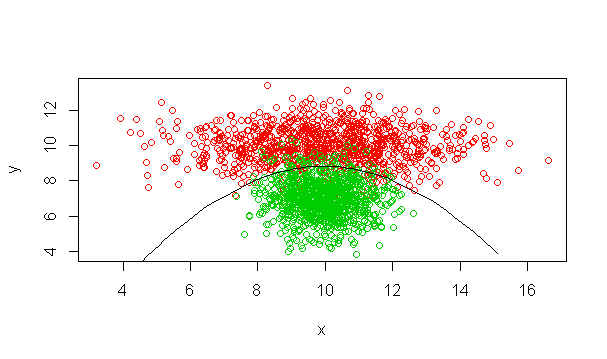
\includegraphics[width=0.7\linewidth]{classes-bonito}
\caption{E as classificamos de acordo com o modelo}

\label{fig:classes-bonito}
\end{figure}

	\end{frame}
	\begin{frame}
		\frametitle{Bayesiano}
		\begin{figure}
\centering
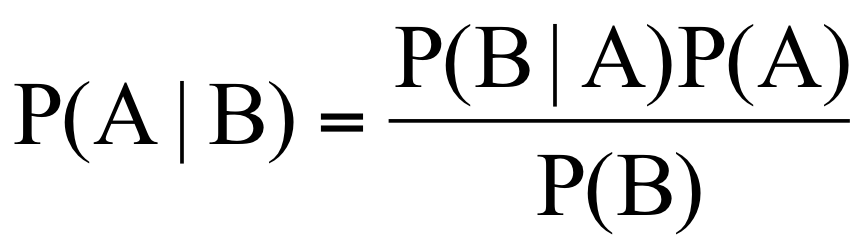
\includegraphics[width=0.7\linewidth]{bayes-limpo}
\caption{O teorema (ou regra) de Bayes}
\label{fig:bayes-limpo}
\end{figure}

	\end{frame}
	\begin{frame}
		\frametitle{CBI - vetor de características}
		\begin{itemize}
			\item Para atribuir a probabilidade de uma palavra (p) pertencer a uma categoria (c), ou seja, para calcular P(c|p), o modelo trata cada palavra como um vetor de traços ($\bar{p}$).\\
			\item Esses traços são as variáveis observadas.\\
			\item Cada valor possível de cada traço tem uma probabilidade relacionada a cada categoria possível.\\
			\item Essas probabilidades são extraídas do corpus.\\
		\end{itemize}
	\end{frame}	

	\begin{frame}
		\frametitle{Ingênuo}
			\begin{itemize}
				\item Ingênuo pois assume que as diversas características observadas não possuem relação nenhuma entre si.\\
				\item Essa não é uma afirmação necessariamente verdadeira, mas...\\
				\item  Isso simplifica o modelo em termos de implementação e computação.\\
		\end{itemize}
	\end{frame}
	\begin{frame}
		\frametitle{CBI - formalização}
		\begin{itemize}
			\item Usando a regra de bayes para calcular P(c|$\bar{p}$), temos que:\\
			\begin{itemize}
				\item[1] P(c|$\bar{p}$) = $\dfrac{P(\bar{p}|c)\times P(c)}{P(\bar{p})}$
				\item[2] E o classificador funciona da seguinte maneira: ele me retorna a classe \textit{c} do conjunto de classes possíveis \textit{C} que maximiza essa probabilidade.\\
				\item CBI($\bar{p}$) = argmax P(c|$\bar{p}$) : ${c\in C}$\\
				\item[3] Isso resulta em uma simplificação da regra de Bayes, pois toda vez que uma classe \textit{c} maximize a função em \textit{1}, ele irá maximizar a função em 4.\\
				\item[4] CBI($\bar{p}$) = argmax (P($\bar{p}|c) \times P(c)$ )
			\end{itemize}
		\end{itemize}
	\end{frame}
	\begin{frame}
		\frametitle{CBI - formalização}
		
		\begin{figure}
\centering
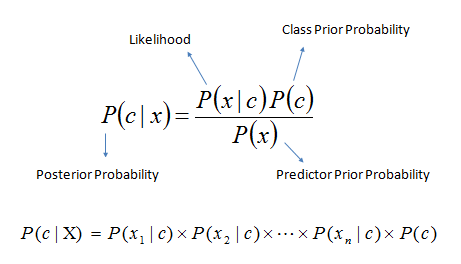
\includegraphics[width=0.7\linewidth]{bayes}
\caption{Probabilidade de um vetor é igual ao produto da probabilidade de cada um dos elementos do vetor dada a categoria \textit{c} em questão.}
\label{fig:bayes}
\end{figure}

	\end{frame}
	\begin{frame}
		\frametitle{Exemplo}
		\begin{itemize}
			\item Palavra: 'perna'\\
			\item Vetor de traços: [Categoria morfossintática: 'Nome', peso da sílaba final: 'leve', nivel de frequência no corpus: 3]\\
			\item Probabilidades:
			\begin{itemize}
				\item Oxítona = p(oxítona)* p('nome'|oxítona) * p('leve'|oxítona)...
				\item Paroxítona = p(paroxítona)* p('nome'|paroxítona) * p('leve'|paroxítona)...
				\item Proparoxítona = p(proparoxítona)* p('nome'|proparoxítona) * p('leve'|proparoxítona)...
			\end{itemize}
			\item Repare que os meus \textit{priors} vão favorecer as categorias paroxítona, oxítona e proparoxítona nessa ordem.\\
			
		\end{itemize}	
	\end{frame}
	\begin{frame}
		\frametitle{Implementação}
		\begin{itemize}
			\item Corpus utilizado: ABG $\rightarrow$ 98.000 palavras.\\
			\item Implementação feita em Python.\\
			\item Foi efeituada uma \textit{Cross-validation} dos resultados.\\
			\item Acertos e erros em comparação com acentuação categórica já presente no corpus.\\
		\end{itemize}
	\end{frame}

%%%%%%%%%%%%%%%%%%%%%%%%%%%%%%%%%%%%%%%%%%%%%%
	\section{Resultados}
	\begin{frame}
		\centering \textbf{Resultados}
	\end{frame}
	\begin{frame}
		\frametitle{Resultados - CBI}
		\begin{itemize}

			\item P = Peso Silábico\\
			\item L = Nível de frequência\\
			\item C = Categoria Morfossintática\\
			\item E = Estrutura silábica (CV-CV)\\
		\end{itemize}
	\end{frame}
	
	\begin{frame}
		\frametitle{Resutlados CBI}
		\begin{figure}
\centering
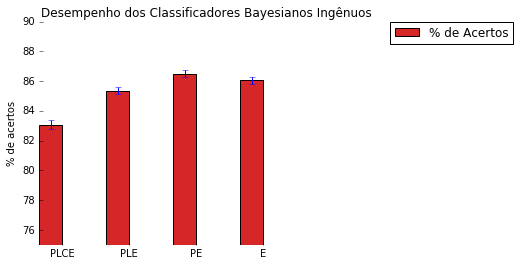
\includegraphics[width=0.9\linewidth]{resultadosnbc}
\label{fig:resultadosnbc}
\end{figure}

	\end{frame}
	\begin{frame}
		\frametitle{Tabela - CBI}
		\begin{table}[]
			\centering
			\caption{Resultados do Classificador Bayesiano Ingênuo}
			\label{my-label}
			\begin{tabular}{@{}lll@{}}
				\toprule
				Parâmetros & Média & Desvio \\ \midrule
				P,L,C,E    & 83.08 & 0.33   \\
				P.L.E      & 85.36 & 0.25   \\
				\textbf{P.E}        & \textbf{86.51} & \textbf{0.26}   \\
				E          & 86.05 & 0.26   \\ \bottomrule
			\end{tabular}
		\end{table}
	\end{frame}
	\begin{frame}
		\frametitle{Resultados - Geral}
		\begin{figure}
\centering
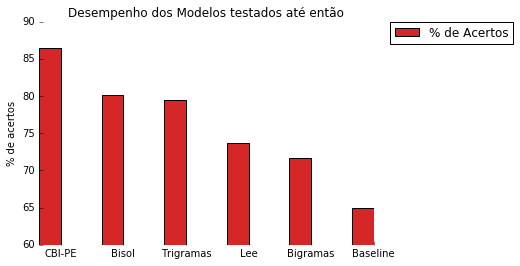
\includegraphics[width=0.9\linewidth]{resultadosgeral}
\label{fig:resultadosgeral}
\end{figure}

	\end{frame}
	\begin{frame}
		\frametitle{Tabela: Desempenho geral}
		\begin{table}[]
			\centering
			\caption{Desempenho Geral}
			\label{my-label}
			\begin{tabular}{@{}ll@{}}
				\toprule
				Parâmetros & Média \\ \midrule
				CBI P.E    & 86.51 \\
				Bisol      & 80.10 \\
				Trigramas  & 79.40 \\
				Lee        & 73.71 \\
				Bigramas   & 71.69 \\
				Baseline   & 65.59 \\ \bottomrule
			\end{tabular}
		\end{table}
	\end{frame}
	
%%%%%%%%%%%%%%%%%%%%%%%%%%%%%%%
	\section{Perspectivas}
	%22
		\begin{frame}
			\centering \textbf{Perspectivas}
		\end{frame}
	\begin{frame}
		\frametitle{Próximos passos}
		\begin{itemize}
			\item Incluir outras versões desse modelo na análise e selecionar as melhores.\\
			\item Escrever, escrever, escrever...\\
		\end{itemize}
	\end{frame}
	%23
	\begin{frame}
		\frametitle{Agradecimento}
		Muito Obrigado!
		
	\end{frame}
\end{document}